\chapter{Eliminação Gaussiana}
\label{cap:eliminação}

\textbf{Importante:} este capítulo é baseado em \cite{slide2doyuri}.

No capítulo anterior, nós entendemos a interpretação geométrica de um sistema linear, e vimos que todo sistema linear pode ser escrito como uma equação matricial $Ax = b$. Agora, nós estamos interessados em encontrar um algoritmo que seja capaz de resolver qualquer sistema linear PD, independentemente do seu tamanho.

\section{Eliminação}

Para descrevermos o processo de eliminação, primeiramente nós vamos definir o que é um pivô. Para motivar este conceito, vamos introduzir qual é a ideia da eliminação. Suponha que nós temos um sistema linear

$$
\begin{cases}
	2x + y = 8 \\
	6x - y = 16
\end{cases}
$$

Olhando geometricamente para este sistema, nós temos a seguinte situação:

\begin{figure}[H]
	\centering
	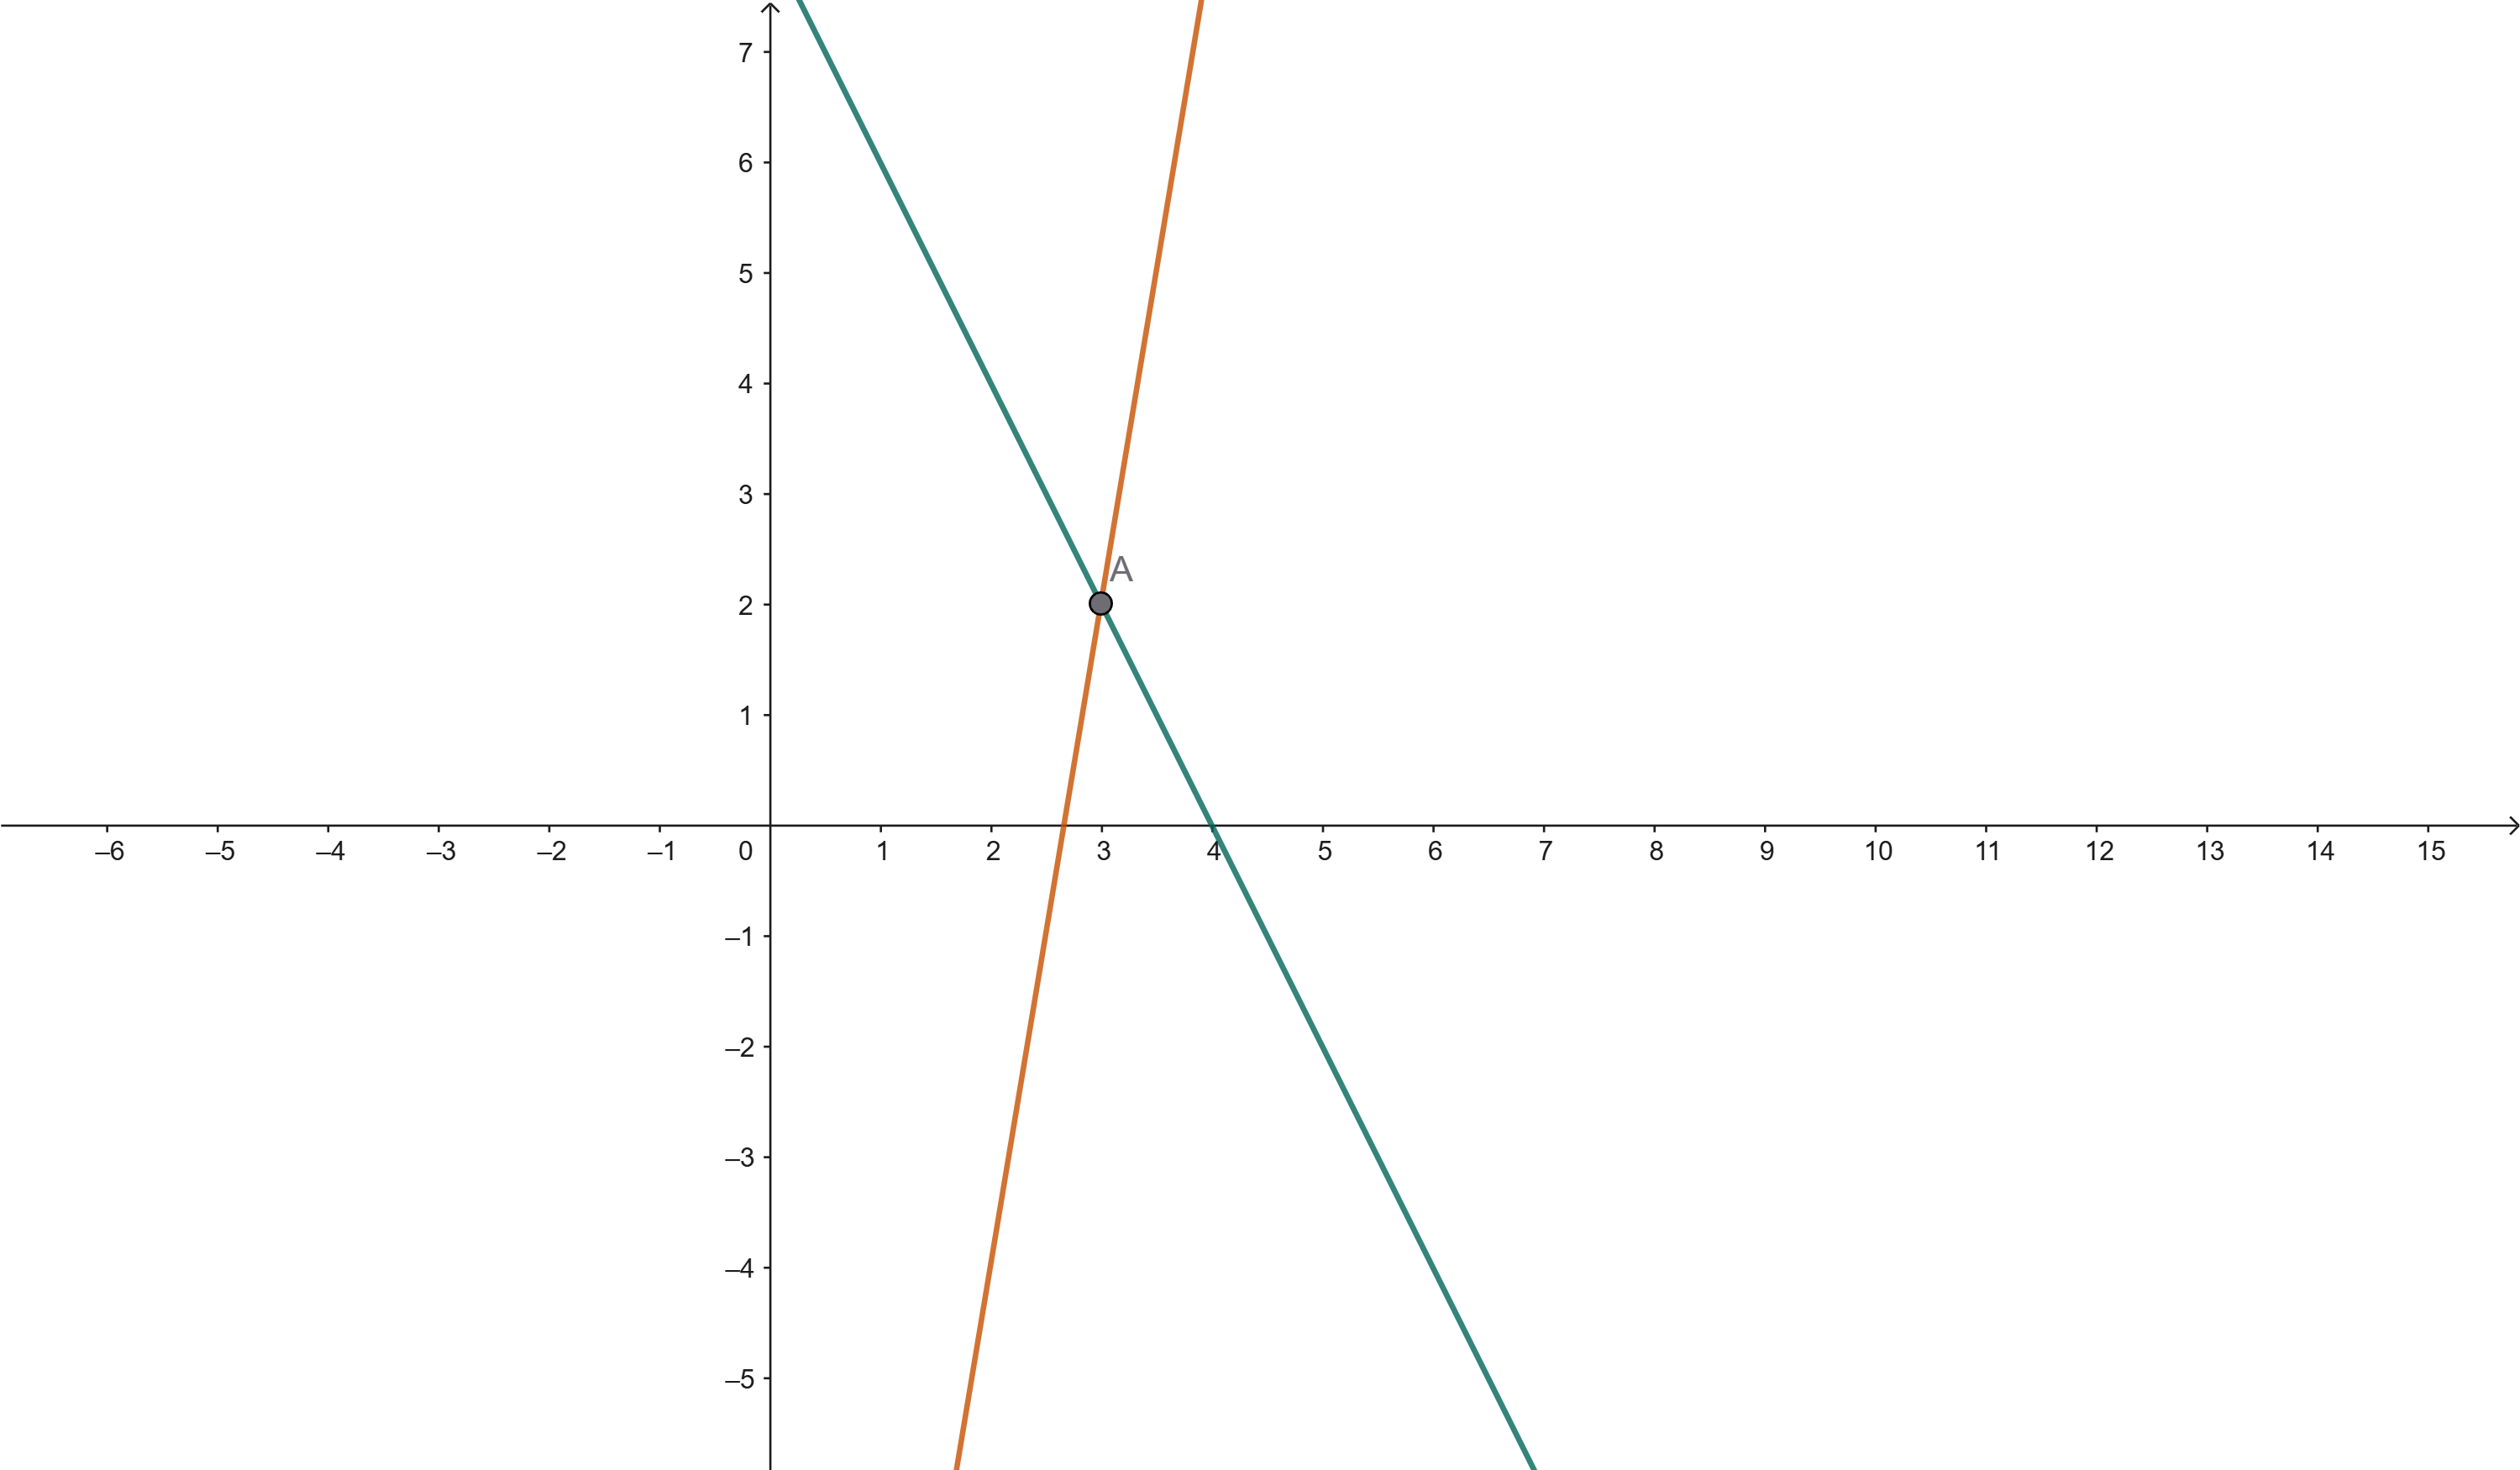
\includegraphics[width=1.0\linewidth]{imgs/alglin-04-eliminacao-1}
	\caption[Sistema linear antes da eliminação]{sistema linear antes da eliminação (arquivo pessoal)}
	\label{fig:alglin-04-eliminacao-1}
\end{figure}

Suponha agora que nós fazemos uma operação nas linhas do sistema: subtraímos 3 vezes a linha 1 da linha 2. Ou seja:

$$
\begin{cases}
	2x + y = 8 \\
	6x - y = 16
\end{cases} \overset{L_2 - 3L_1}{\implies} \begin{cases}
	2x + y = 8 \\
	~~~-4y = -8
\end{cases}
$$

Segue que $y = 2$ e $x = 3$ no segundo sistema. Porém, veja o que acontece geometricamente quando fazemos esta operação:

\begin{figure}[H]
	\centering
	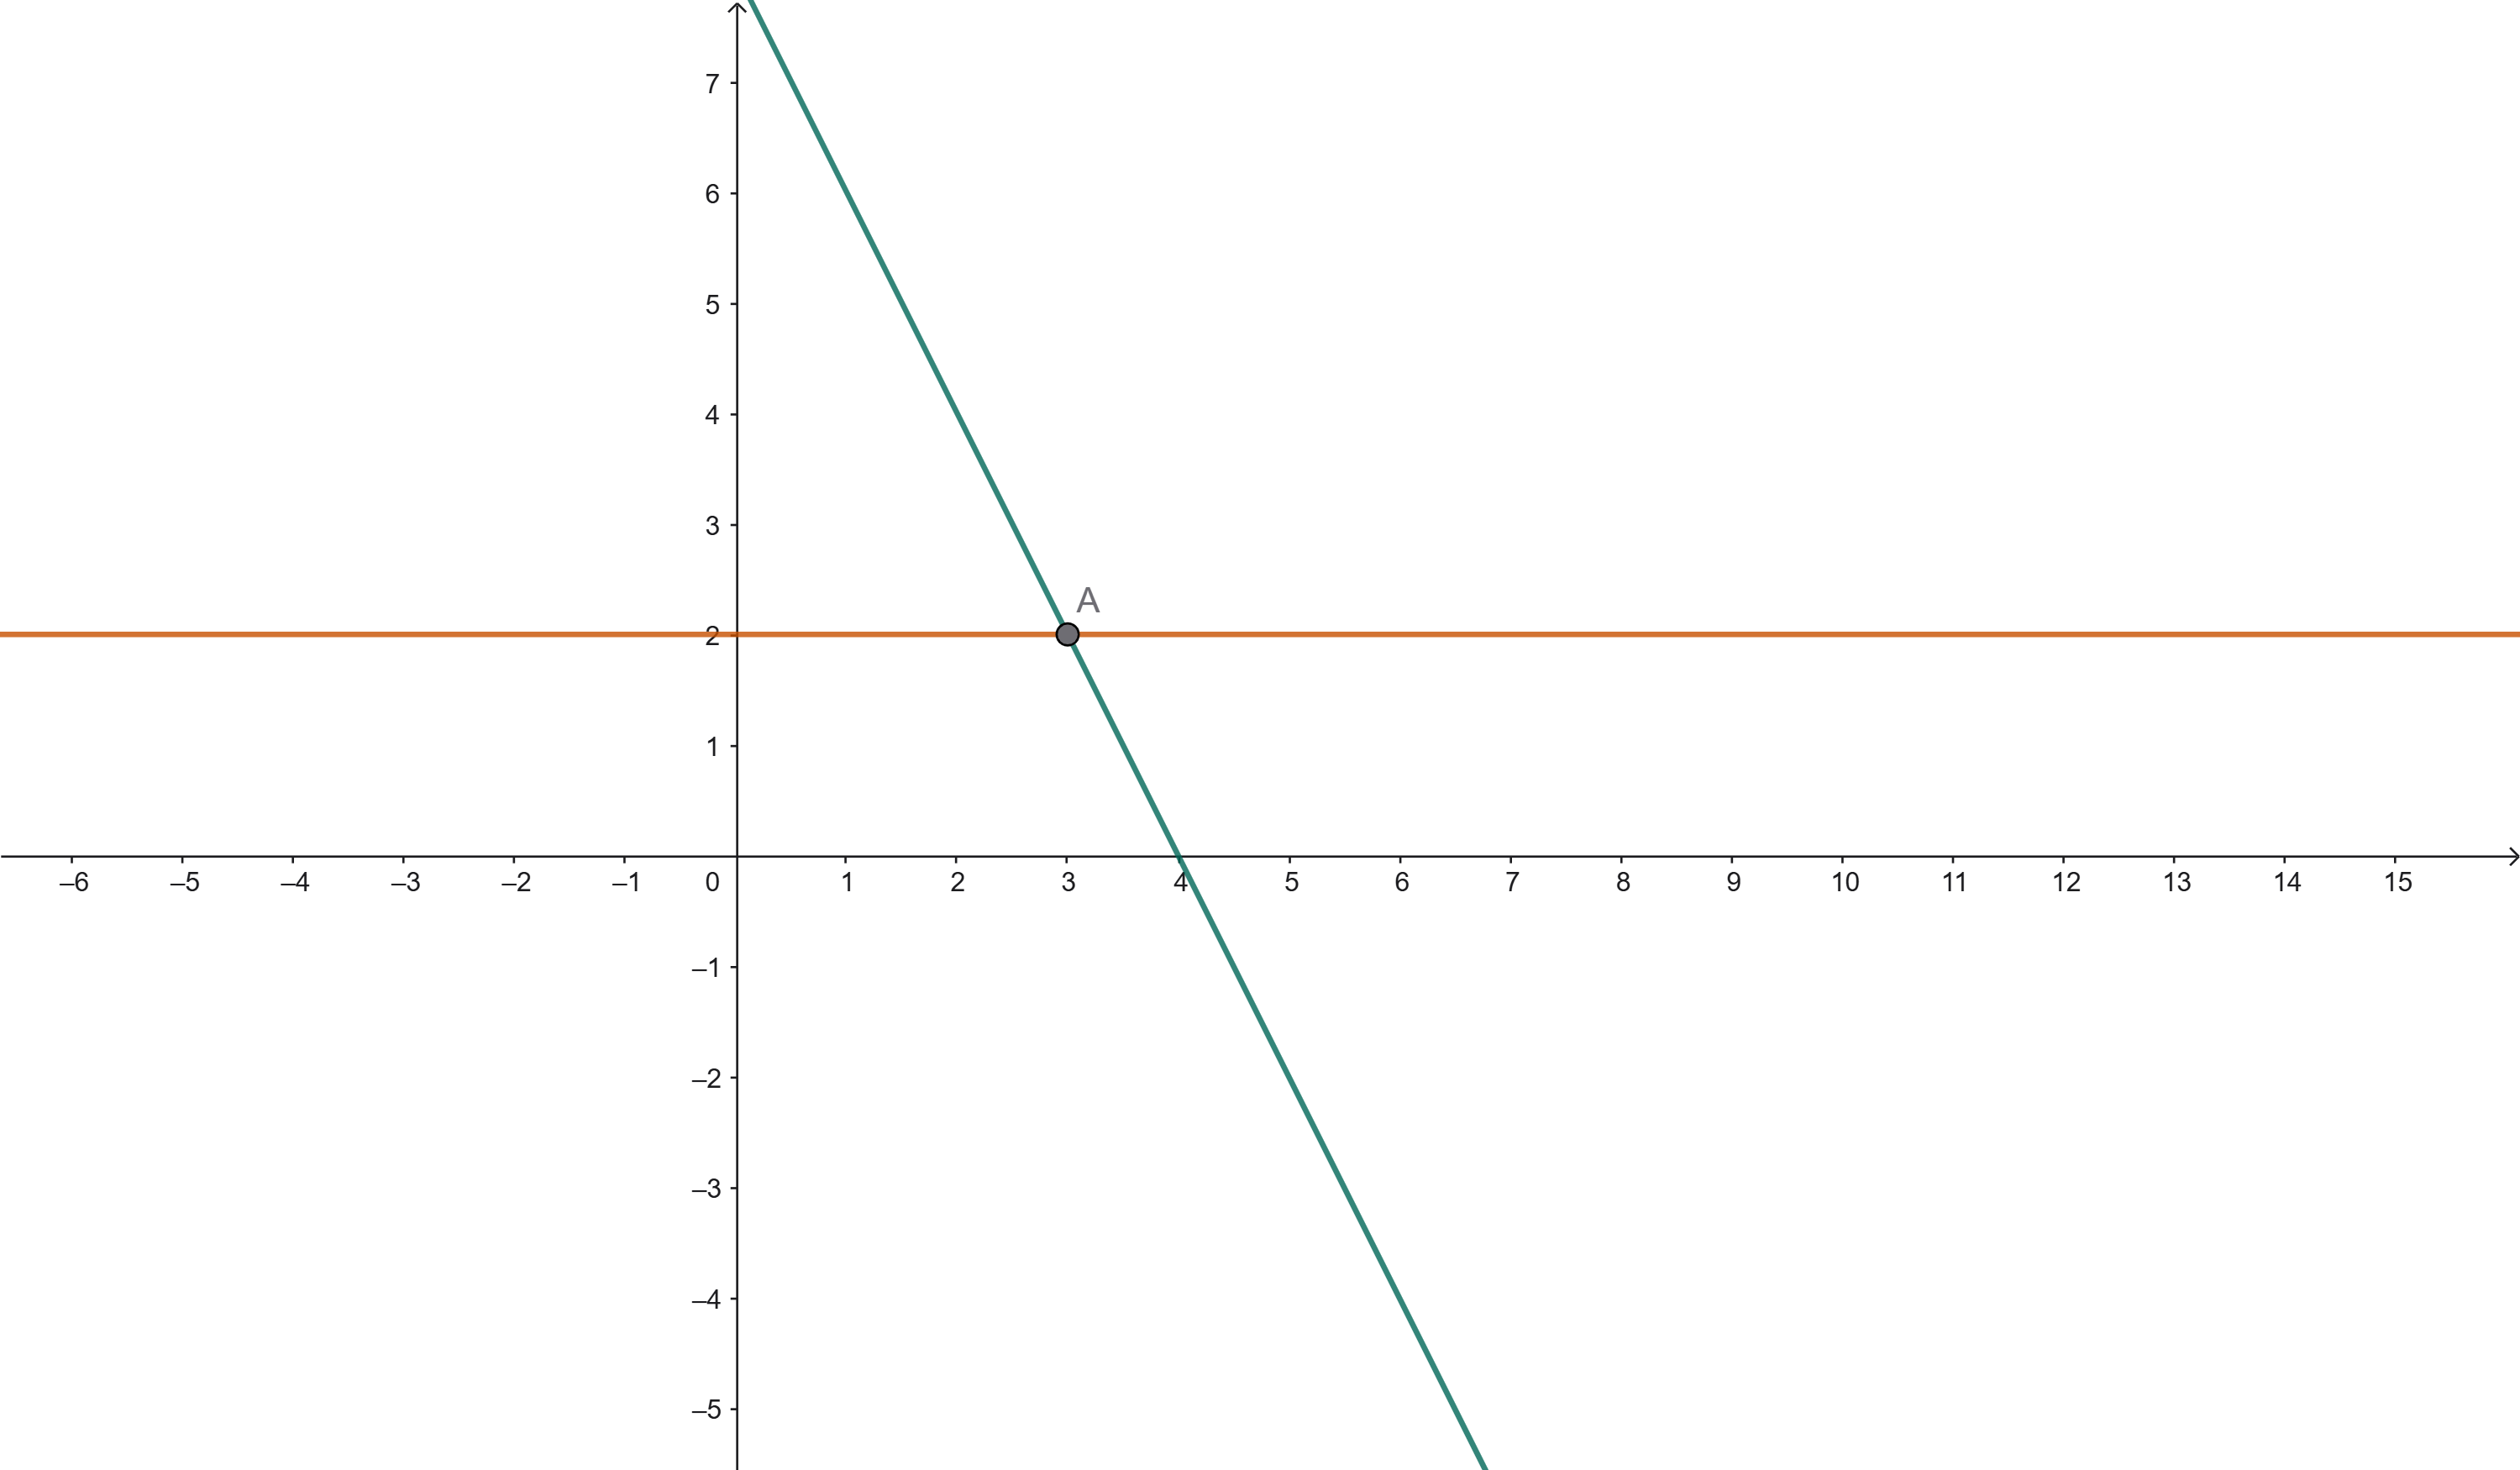
\includegraphics[width=1.0\linewidth]{imgs/alglin-05-eliminacao-2}
	\caption[Sistema linear depois da eliminação]{sistema linear depois da eliminação (arquivo pessoal)}
	\label{fig:alglin-05-eliminacao-2}
\end{figure}

Como podemos perceber, a solução do segundo sistema linear é também a solução do primeiro sistema. Então, se nós tivermos um sistema linear PD mais complexo, a ideia é que nós podemos resolvê-lo facilmente apenas utilizando somas, multiplicações e (como nós veremos) trocas de linha.

No entanto, como nós vimos no primeiro capítulo, nem todo sistema linear é possível e determinado. Alguns sistemas não possuem nenhuma solução, e outros sistemas possuem infinitas soluções. Vamos ver o que acontece no caso $2\times 2$ quando aplicamos a eliminação nesses tipos de sistemas.

\begin{Example}
	Considere o sistema linear
	
	$$
	\begin{cases}
		2x + y = 3 \\
		4x + 2y = 7
	\end{cases}
	$$
	
	Este sistema, como se pode perceber facilmente, não possui nenhuma solução. Se fizermos $L_2 - 2L_1$, nós obtemos:
	
	$$
	\begin{cases}
		2x + y = 3 \\
		0x + 0y = 1
	\end{cases}
	$$
	
	Ou seja, nós zeramos o lado esquerdo da segunda equação, mas obtivemos $0 = 1$, o que é um absurdo. Isso justifica o fato de o sistema não possuir nenhuma solução.
\end{Example}

\begin{Example}
	Considere o sistema linear
	
	$$
	\begin{cases}
		2x + y = 3 \\
		4x + 2y = 6
	\end{cases}
	$$
	
	Também é fácil observar o que acontece com este sistema: como a segunda linha é múltipla da primeira, qualquer ponto que satisfaça à primeira equação satisfará também a segunda, logo, este sistema possui infinitas soluções. Se fizermos $L_2 - 2L_1$, nós obteremos:
	
	$$
	\begin{cases}
		2x + y = 3 \\
		0x + 0y = 0
	\end{cases}
	$$
	
	Ou seja, nós zeramos a linha 2 inteira, obtendo $0 = 0$. Isso justifica o fato de o sistema possuir infinitas soluções.
\end{Example}

Em ambos os casos, quando o sistema é impossível, e quando o sistema é possível e indeterminado, a eliminação produz uma linha inteira de zeros no lado esquerdo da equação. Por outro lado, quando o sistema é possível e determinado, isso não acontece. Então, a partir deste fato, nós podemos definir o conceito de pivô:

\begin{Definition}
	Nós chamamos de \textbf{pivô} ao primeiro elemento não-nulo de uma linha usado para eliminação.
\end{Definition}

% Melhorar a definição

É importante notar que os pivôs não são considerados em relação ao estado inicial do sistema, mas em relação ao seu estado final. Isso quer dizer que, a cada passo da eliminação, nós obtemos um novo pivô (se o sistema for possível e determinado).

Por exemplo, no primeiro sistema de equações deste capítulo, os pivôs são $2$ e $-4$. Já nos dois sistemas seguintes, o único pivô é $2$. Isso nos leva a uma consequência importante: se o sistema possui $n$ equações e menos de $n$ pivôs, ou ele não possui solução, ou ele possui infinitas soluções. Por outro lado, se o sistema possui $n$ equações e $n$ pivôs, ele possui exatamente uma solução, mas pode ser necessário trocar linhas durante o processo de eliminação.

Uma pergunta importante é: "como nós definimos o fator de multiplicação durante o processo de eliminação?". Como, por exemplo, eu pude falar no primeiro sistema do capítulo que faríamos "$L_2 - 3L_1$"? De fato, a cada passo da eliminação, o que nós queremos produzir zeros imediatamente abaixo do pivô, de modo que, ao final, a última linha fique com apenas 1 termo diferente de zero, a penúltima fique com 2 termos diferentes de zero, e assim sucessivamente até a primeira linha, que permanece inalterada.

Para fazer isso, nós podemos definir o multiplicador como abaixo:

\begin{Definition}
	Nós definimos o \textbf{multiplicador} como:
	
	$$
	\text{multiplicador} = \dfrac{\text{elemento a ser eliminado}}{\text{pivô}}.
	$$
\end{Definition}
